\documentclass[aspectratio=169]{beamer}
\mode<presentation>

\usepackage{adjustbox}
\usepackage{array}
\usepackage{calc}
\usepackage{etoolbox}
\usepackage{fancyvrb}
\usepackage{listings}
\usepackage{relsize}
\usepackage{graphicx}
\usepackage[most]{tcolorbox}
\usepackage[overlay,absolute]{textpos}
\usepackage{xcolor}

\usepackage{tikz}
\usetikzlibrary{arrows.meta}
\usetikzlibrary{positioning}
\usetikzlibrary{tikzmark}

\graphicspath{{../images}}

\usepackage{fontspec}
\setsansfont{Helvetica Neue Light}[
    BoldFont={Helvetica Neue Bold},
    BoldItalicFont={Helvetica Neue Bold Italic},
    ItalicFont={Helvetica Neue Light Italic}
]
\setmonofont{Iosevka Term}
\newfontface\helvreg{Helvetica Neue}

\definecolor{grayish}{gray}{0.8}

\title{Concatenative programming and stack-based languages}
\author{Douglas Creager}
\institute{Walland Heavy Research}

\setbeamercolor{title}{fg=black}
\setbeamerfont{title}{series=\bfseries,size=\larger[1]}
\setbeamerfont{subtitle}{series=\mdseries,size=\smaller[2]}
\setbeamerfont{author}{size=\smaller[1]}
\setbeamerfont{institute}{size=\smaller[2]}
\setbeamertemplate{navigation symbols}{}
\setbeamercolor{frametitle}{fg=black}
\setbeamerfont{frametitle}{series=\bfseries}

% Picture credits

\makeatletter
\def\picturecredits{}
\newcommand{\picturecredit}[4]{
    \protected@xappto\picturecredits{
        \textsmaller[3]{Slide \theframenumber} &
        \textsmaller[2]{#1, “#2”} \vspace*{-0.4em} \newline
        \ifstrempty{#4}{\textsmaller[3]{#3}}{\textsmaller[3]{#3, \url{#4}}} \\
    }
}
\makeatother

\newlength{\titlewidth}
\newcommand{\customtitle}[3]{
    \settowidth{\titlewidth}{#3}
    \begin{textblock*}{\titlewidth}(#1,#2)
        #3
    \end{textblock*}
}
\newcommand{\flattitle}[3]{\customtitle{#1}{#2}{\textbf{\LARGE #3}}}

\newcommand{\customshadowedtitle}[4]{
    \settowidth{\titlewidth}{#4}
    \addtolength{\titlewidth}{#3}
    \addtolength{\titlewidth}{0.1mm}
    \begin{textblock*}{\titlewidth}(#3+#1,#3+#2)
        #4
    \end{textblock*}
    \begin{textblock*}{\titlewidth}(#1,#2)
        \textcolor{white}{#4}
    \end{textblock*}
}
\newcommand{\shadowedtitle}[3]{\customshadowedtitle{#1}{#2}{0.4mm}{\textbf{\LARGE #3}}}

%%%%%%%%%%%%%%%%%%%%%%%%%%%%%%%%%%%%%%%%%%%%%%%%%%%%%%%%%%%%%%%%%%%%%%%%%%%%%%%%
% True centering of beamer slides

\makeatletter
\define@key{beamerframe}{c}[true]{% centered
  \beamer@frametopskip=0pt plus 1fill\relax%
  \beamer@framebottomskip=0pt plus 1fill\relax%
  \beamer@frametopskipautobreak=0pt plus .4\paperheight\relax%
  \beamer@framebottomskipautobreak=0pt plus .6\paperheight\relax%
  \def\beamer@initfirstlineunskip{}%
}
\makeatother

%%%%%%%%%%%%%%%%%%%%%%%%%%%%%%%%%%%%%%%%%%%%%%%%%%%%%%%%%%%%%%%%%%%%%%%%%%%%%%%%
% Explicit control of overlay-style visibility

% cf https://tex.stackexchange.com/a/512131

\makeatletter
\newcommand\pgfinvisible{\pgfsys@begininvisible}
\newcommand\pgfshown{\pgfsys@endinvisible}
\makeatother

%%%%%%%%%%%%%%%%%%%%%%%%%%%%%%%%%%%%%%%%%%%%%%%%%%%%%%%%%%%%%%%%%%%%%%%%%%%%%%%%
% Program source

\lstset{
  basicstyle=\small\ttfamily,%
  columns=fullflexible,
  keepspaces=true,
  escapechar=?,
  extendedchars=true}

\newcommand{\highlightsrc}[1]{%
    \tikz[remember picture]{
      \draw [overlay, draw=none, fill=blue!25]
        ([xshift=-1pt, yshift=8pt] pic cs:#1_start)
        rectangle
        ([xshift=1pt, yshift=-2pt] pic cs:#1_end)
        ;
    }%
    \ignorespaces
}

%%%%%%%%%%%%%%%%%%%%%%%%%%%%%%%%%%%%%%%%%%%%%%%%%%%%%%%%%%%%%%%%%%%%%%%%%%%%%%%%
% Environment frames

% Note that to use beamer overlays to ADD NEW rows to a tikz matrix, you need to
% put the TRAILING ROW'S closing \\ inside the \only, instead of the NEW ROW'S.
% c.f. https://tex.stackexchange.com/a/153797

\tikzset{
    envframe/.style={
        ampersand replacement=\&,
        draw=black,
        thick,
        rounded corners,
        fill=white,
        inner ysep=0.1em,
        row sep=-0.1em,
        every outer matrix/.append style={inner xsep=0.2em,inner ysep=0.2em},
        column 1/.style={
            sharp corners,
            anchor=base west,
        },
        column 2/.style={
            anchor=base,
            font=\small,
        },
    },
}

\tikzset{
    frame name/.style={
        execute at end node=\strut,
        font=\ttfamily\footnotesize\bfseries,
    },
    frame special/.style={
        execute at end node=\strut,
        font=\itshape\scriptsize,
    },
}

\tikzset{
    highlight node/.style={fill=red!25},
    highlight node on/.code args={<#1>}{%
        \alt<#1>{\pgfkeysalso{highlight node}}{}%
    }
}

%%%%%%%%%%%%%%%%%%%%%%%%%%%%%%%%%%%%%%%%%%%%%%%%%%%%%%%%%%%%%%%%%%%%%%%%%%%%%%%%
% Simple stack language

\newdimen\origiwspc
\origiwspc=\fontdimen2\font

\newcommand<>{\stackex}[2]{%
    \begin{onlyenv}#3
    \begin{tabular}[c]{
        @{\extracolsep{1em}}
        >{\rule[-0.6\baselineskip]{0pt}{1.8\baselineskip}\raggedleft\arraybackslash\fontdimen2\font=1ex}p{0.4\textwidth}<{\fontdimen2\font=\origiwspc}
        |
        >{\strut\raggedright\arraybackslash\leavevmode\color{blue}\ttfamily}p{0.5\textwidth}
    }
        \cline{1-1}
        \clipbox*{{\width - 0.4\textwidth} {-\depth} {\width} {\totalheight}}{#1} &
        \clipbox*{0pt {-\depth} {0.5\textwidth} {\totalheight}}{#2} \\
        \cline{1-1}
    \end{tabular}
    \end{onlyenv}%
    \ignorespaces
}

\newcommand{\sym}[1]{\textcolor{blue}{\texttt{#1}}}
\newcommand{\quot}[1]{\textcolor{blue}{\texttt{[#1]}}}
\newcommand{\eff}[1]{\textcolor{gray}{\texttt{\textit{#1}}}}

\newcommand{\stacksplit}[2][]{%
    \tcbox[
        standard jigsaw,
        nobeforeafter,
        size=fbox,
        boxrule=0pt,
        sharp corners=all,
        colback=white!0,
        #1
    ]{\sym{\strut#2}}%
    \ignorespaces
}

\newcommand{\stackeffect}[2]{%
    \hspace{\fill}%
    \begin{tikzpicture}
        \matrix[
            anchor=west,
            execute at begin cell=\node\bgroup,
            execute at end cell=\egroup;%
        ]{
            \eff{#1} \\
            \sym{#2} \\
        };
    \end{tikzpicture}%
    \hspace*{\fill}%
    \ignorespaces
}

%%%%%%%%%%%%%%%%%%%%%%%%%%%%%%%%%%%%%%%%%%%%%%%%%%%%%%%%%%%%%%%%%%%%%%%%%%%%%%%%
% Citations

\newcommand<>{\citepaper}[1]{%
    \begin{onlyenv}#2%
    \begin{tikzpicture}[remember picture,overlay]
        \node[
            anchor=south, yshift=1em,
            draw, thick,
            inner sep=0.6em,
            text width=90mm,
            node font={\rmfamily\smaller[2]},
        ] at (current page.south) {#1};
    \end{tikzpicture}%
    \end{onlyenv}%
    \ignorespaces
}

%%%%%%%%%%%%%%%%%%%%%%%%%%%%%%%%%%%%%%%%%%%%%%%%%%%%%%%%%%%%%%%%%%%%%%%%%%%%%%%%

\begin{document}

\begin{frame}
    \begin{textblock*}{160mm}(0mm,0mm)
        \picturecredit{Douglas Creager}{Laurel Valley}{All rights reserved}{}
        \adjincludegraphics[Trim=13.5in 0.25in 15in 11in, width=160mm]{laurel-valley.jpg}
    \end{textblock*}
    \customshadowedtitle{80mm - 0.5\titlewidth}{61mm}{0.2mm}{\textbf{\textlarger[1]{\inserttitle}}}
    \customshadowedtitle{80mm - 0.5\titlewidth}{69mm}{0.2mm}{\textsmaller[1]{\insertauthor}}
    \customshadowedtitle{80mm - 0.5\titlewidth}{73mm}{0.2mm}{\textsmaller[2]{\insertinstitute}}
    \customshadowedtitle{80mm - 0.5\titlewidth}{79mm}{0.2mm}{\textsmaller[2]{Strange Loop – Papers We Love}}
    \customshadowedtitle{80mm - 0.5\titlewidth}{82.5mm}{0.2mm}{\textsmaller[3]{September 21–22, 2023 – St. Louis}}
\end{frame}

%%%%%%%%%%%%%%%%%%%%%%%%%%%%%%%%%%%%%%%%%%%%%%%%%%%%%%%%%%%%%%%%%%%%%%%%%%%%%%%%
% Initial stack language examples

\begin{frame}
    \begin{textblock*}{160mm}(0mm,0mm)
        \picturecredit{peagreengirl}{Very Old payroll Journal}{CC-BY-2.0}{https://flic.kr/p/B2YPU}
        \adjincludegraphics[Trim=0.25in, width=160mm]{old-ledger.jpg}
    \end{textblock*}
    \shadowedtitle{150mm - \titlewidth}{10mm}{Names}
\end{frame}

\begin{frame}[fragile]
    \frametitle{Pythagoras}
    \begin{columns}[c]
        \begin{column}{90mm}%
        \centering%
        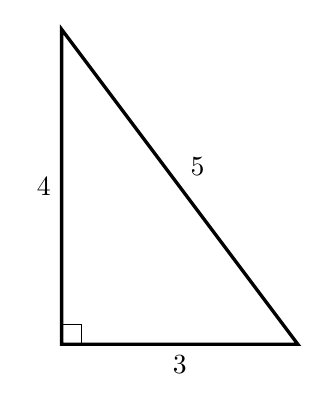
\begin{tikzpicture}[baseline={(current bounding box.center)}]
            \draw[very thick]
              (0,0) -- node[left] {4}
              (0,4) -- node[above right] {5}
              (3,0) -- node[below] {3} cycle;
            \draw[thin] (0,0.25) -- (0.25,0.25) -- (0.25,0);
        \end{tikzpicture}
        \end{column}%
        \begin{column}{70mm}%
        \begin{onlyenv}<1-2>%
        \begin{lstlisting}[language=python,gobble=8]
        import math

        leg1 = 3
        leg2 = 4

        l1sq = leg1 * leg1
        l2sq = leg2 * leg2
        hypotsq = l1sq + l2sq
        result = math.sqrt(hypotsq)

        print(result)
        \end{lstlisting}%
        \begin{uncoverenv}<2>%
        \begin{lstlisting}[gobble=8,basicstyle={\color{blue}\ttfamily\larger[1]}]
        5
        \end{lstlisting}%
        \end{uncoverenv}%
        \end{onlyenv}%
        \begin{onlyenv}<3>%
        \begin{lstlisting}[language=python,gobble=8]
        import math

        def pythogoras(leg1, leg2):
            l1sq = leg1 * leg1
            l2sq = leg2 * leg2
            hypotsq = l1sq + l2sq
            return math.sqrt(hypotsq)

        print(pythagoras(3, 4))
        print(pythagoras(5, 12))
        \end{lstlisting}%
        \pgfinvisible%
        \begin{lstlisting}[gobble=8,basicstyle={\color{blue}\ttfamily\larger[1]},belowskip=0pt]
        5
        \end{lstlisting}%
        \begin{lstlisting}[gobble=8,basicstyle={\color{blue}\ttfamily\larger[1]},aboveskip=0pt]
        13
        \end{lstlisting}%
        \pgfshown%
        \end{onlyenv}%
        \end{column}%
    \end{columns}%
\end{frame}

\begin{frame}[fragile]
    \frametitle{Pythagoras}
    \begin{columns}[c]
        \begin{column}{90mm}%
        \only<2-3>  {\highlightsrc{math}}%
        \only<4>    {\highlightsrc{pyth}}%
        \only<5>    {\highlightsrc{formals}}%
        \only<5-9>  {\highlightsrc{actuals1}}%
        \only<6>    {\highlightsrc{s1}}%
        \only<7>    {\highlightsrc{s2}}%
        \only<8>    {\highlightsrc{s3}}%
        \only<9>    {\highlightsrc{s4}}%
        \only<11-15>{\highlightsrc{actuals2}}%
        \only<12>   {\highlightsrc{s1}}%
        \only<13>   {\highlightsrc{s2}}%
        \only<14>   {\highlightsrc{s3}}%
        \only<15>   {\highlightsrc{s4}}%
        \centering%
        \begin{tikzpicture}[
            remember picture,
            every node/.style={node distance=0.5cm},
        ]
        \matrix[envframe] (mod) {
            \only<1>{\node[inner sep=0.6em]{};}
            \only<2- >{
                \node[frame name,highlight node on={<9>}]{math}; \&
                \node[frame special] (math) {math module};
            }
            \only<4- >{ \\
                \node[frame name,highlight node on={<5>}]{pythagoras}; \&
                \node[frame special]{pythagoras function};
            }
            \\
        };
        \only<3- >{
            \matrix[envframe,above=of mod] (mathframe) {
                \& \node{$\cdots$}; \\
                \node[frame name,highlight node on={<9>}]{sqrt}; \&
                \node[frame special]{sqrt function}; \\
                \& \node{$\cdots$}; \\
            };
        }
        \only<3>{
            \draw [overlay, thick, -{Triangle[]}]
              (math.east) .. controls +(0:1cm) and +(0:1cm) ..
              (mathframe.east);
        }
        \only<4- >{
            \draw [overlay, thick, -{Triangle[]}]
              (math.east) .. controls +(0:0.75cm) and +(0:1.25cm) ..
              (mathframe.east);
        }
        \only<5-9>{
            \matrix[envframe,below=of mod] (call1) {
                \only<5-9>{
                    \node[frame name, highlight node on={<6>}]{leg1}; \& \node{3}; \\
                    \node[frame name, highlight node on={<7>}]{leg2}; \& \node{4};
                }
                \only<6-9>{ \\
                    \node[frame name, highlight node on={<8>}]{l1sq}; \& \node{9};
                }
                \only<7-9>{ \\
                    \node[frame name, highlight node on={<8>}]{l2sq}; \& \node{16};
                }
                \only<8-9>{ \\
                    \node[frame name,highlight node on={<9>}]{hypotsq}; \& \node{25};
                }
                \\
            };
            \draw[densely dashed, thick, ->] (call1.north) -- (mod.south);
        }
        \only<11-15>{
            \matrix[envframe,below=of mod] (call1) {
                \only<11-16>{
                    \node[frame name, highlight node on={<12>}]{leg1}; \& \node{5}; \\
                    \node[frame name, highlight node on={<13>}]{leg2}; \& \node{12};
                }
                \only<12-16>{ \\
                    \node[frame name, highlight node on={<14>}]{l1sq}; \& \node{25};
                }
                \only<13-16>{ \\
                    \node[frame name, highlight node on={<14>}]{l2sq}; \& \node{144};
                }
                \only<14-16>{ \\
                    \node[frame name,highlight node on={<15>}]{hypotsq}; \& \node{169};
                }
                \\
            };
            \draw[densely dashed, thick, ->] (call1.north) -- (mod.south);
        }
        \end{tikzpicture}%
        \end{column}%
        \begin{column}{70mm}%
        \begin{lstlisting}[language=python,gobble=8]
        ?\tikzmark{math_start}?import math?\tikzmark{math_end}?

        ?\tikzmark{pyth_start}?def ?\tikzmark{formals_start}?pythogoras(leg1, leg2)?\tikzmark{formals_end}?:
            ?\tikzmark{s1_start}?l1sq = leg1 * leg1?\tikzmark{s1_end}?
            ?\tikzmark{s2_start}?l2sq = leg2 * leg2?\tikzmark{s2_end}?
            ?\tikzmark{s3_start}?hypotsq = l1sq + l2sq?\tikzmark{s3_end}?
            return ?\tikzmark{s4_start}?math.sqrt(hypotsq)?\tikzmark{pyth_end}\tikzmark{s4_end}?

        print(?\tikzmark{actuals1_start}?pythagoras(3, 4)?\tikzmark{actuals1_end}?)
        print(?\tikzmark{actuals2_start}?pythagoras(5, 12)?\tikzmark{actuals2_end}?)
        \end{lstlisting}%
        \begin{uncoverenv}<10->%
        \begin{lstlisting}[gobble=8,basicstyle={\color{blue}\ttfamily\larger[1]},belowskip=0pt]
        5
        \end{lstlisting}%
        \end{uncoverenv}%
        \begin{uncoverenv}<16->%
        \begin{lstlisting}[gobble=8,basicstyle={\color{blue}\ttfamily\larger[1]},aboveskip=0pt]
        13
        \end{lstlisting}%
        \end{uncoverenv}%
        \end{column}%
    \end{columns}%
\end{frame}

\begin{frame}
    \begin{textblock*}{160mm}(0mm,0mm)
        \picturecredit{Marco Verch}{Stack of pancakes with berries on a plate}{CC-BY-2.0}{https://flic.kr/p/2jYUh8M}
        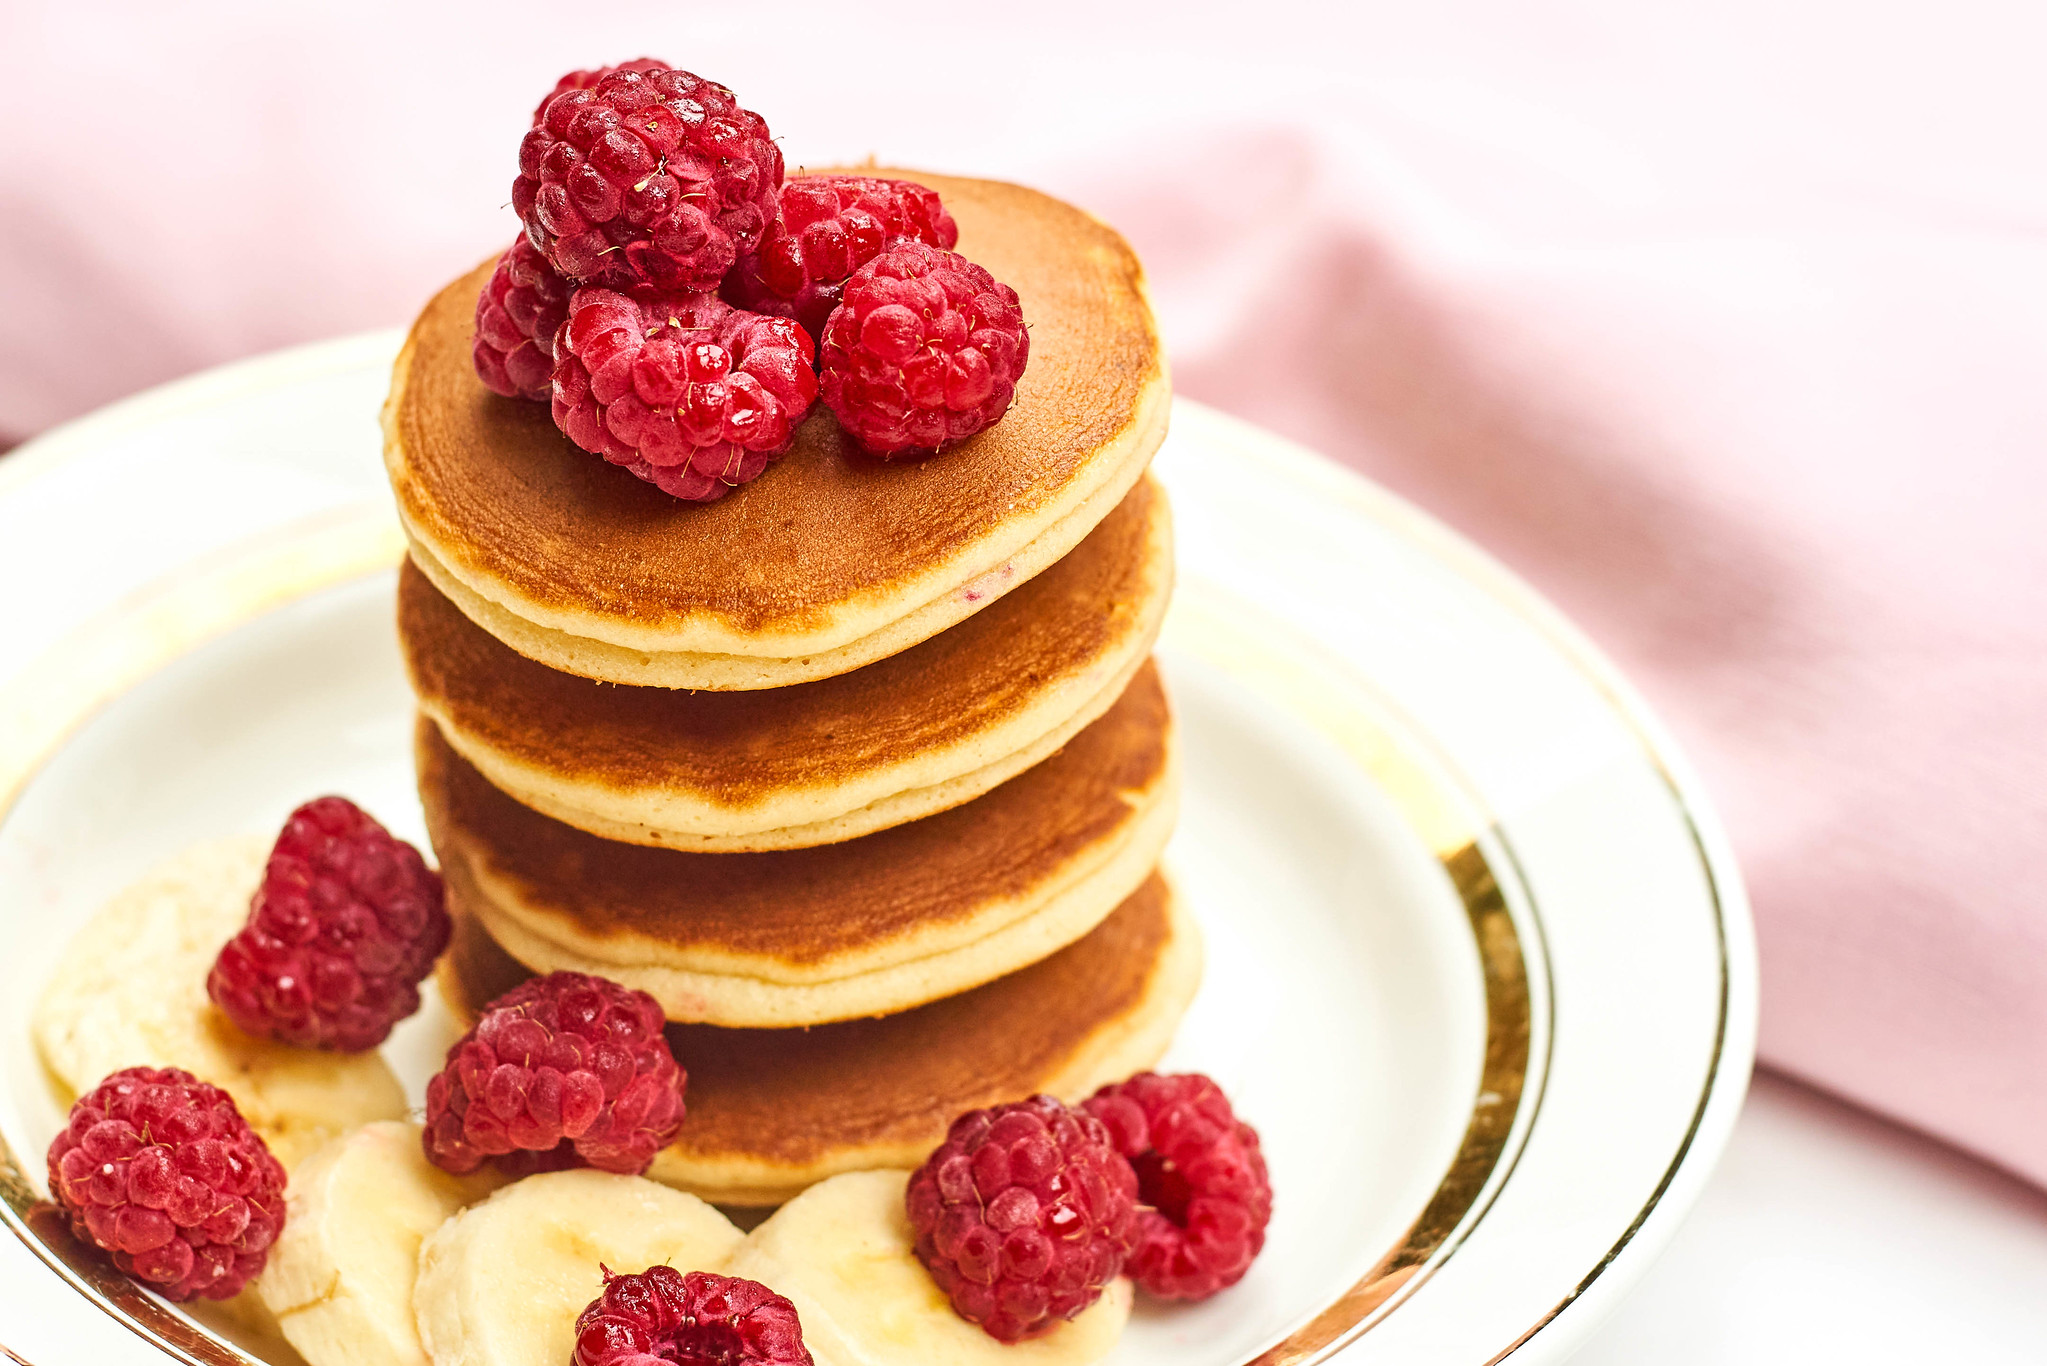
\includegraphics[width=180mm]{pancakes.jpg}
    \end{textblock*}
    \flattitle{150mm - \titlewidth}{5mm}{Stack-based languages}
\end{frame}

\begin{frame}
    \frametitle{Programs operate on a stack}
    \stackex<+>{       }{ }
    \stackex<+>{       }{ 1 2 + }
    \stackex<+>{      1}{ 2 + }
    \stackex<+>{    1 2}{ + }
    \stackex<+>{      3}{ }
\end{frame}

\begin{frame}
    \frametitle{The stack doesn't have to start empty}
    \stackex<+>{  1337 42 1}{ 2 + }
    \stackex<+>{1337 42 1 2}{ + }
    \stackex<+>{  1337 42 3}{ }
\end{frame}

\begin{frame}[fragile]
    \frametitle{Stack effects}
    \stackeffect{i -- result}{2 +}
    \citepaper<2>{
        Slava Pestov, Daniel Ehrenberg, Joe Groff.
        “Factor: A Dynamic Stack-based Programming Language”.
        ACM SIGPLAN Notices 45:12. December 2010.
    }
\end{frame}

\begin{frame}
    \frametitle{Stack underflow is not fatal}
    \stackex<+>{         }{ 2 + }
    \stackex<+>{        2}{ + }
    \stackex<+>{2 \sym{+}}{ }
\end{frame}

\begin{frame}
    \frametitle{Pythagoras}
    \stackex<+>{       }{ 1 2 + 3 * 2 2 + 7 3 - * + sqrt }
    \stackex<+>{      1}{ 2 + 3 * 2 2 + 7 3 - * + sqrt }
    \stackex<+>{    1 2}{ + 3 * 2 2 + 7 3 - * + sqrt }
    \stackex<+>{      3}{ 3 * 2 2 + 7 3 - * + sqrt }
    \stackex<+>{    3 3}{ * 2 2 + 7 3 - * + sqrt }
    \stackex<+>{      9}{ 2 2 + 7 3 - * + sqrt }
    \stackex<+>{    9 2}{ 2 + 7 3 - * + sqrt }
    \stackex<+>{  9 2 2}{ + 7 3 - * + sqrt }
    \stackex<+>{    9 4}{ 7 3 - * + sqrt }
    \stackex<+>{  9 4 7}{ 3 - * + sqrt }
    \stackex<+>{9 4 7 3}{ - * + sqrt }
    \stackex<+>{  9 4 4}{ * + sqrt }
    \stackex<+>{   9 16}{ + sqrt }
    \stackex<+>{     25}{ sqrt }
    \stackex<+->{      5}{ }
    \begin{onlyenv}<+>
        \begin{tikzpicture}[remember picture,overlay]
            \node[anchor=center,draw,thick,inner sep=0mm] at (current page.center) {
                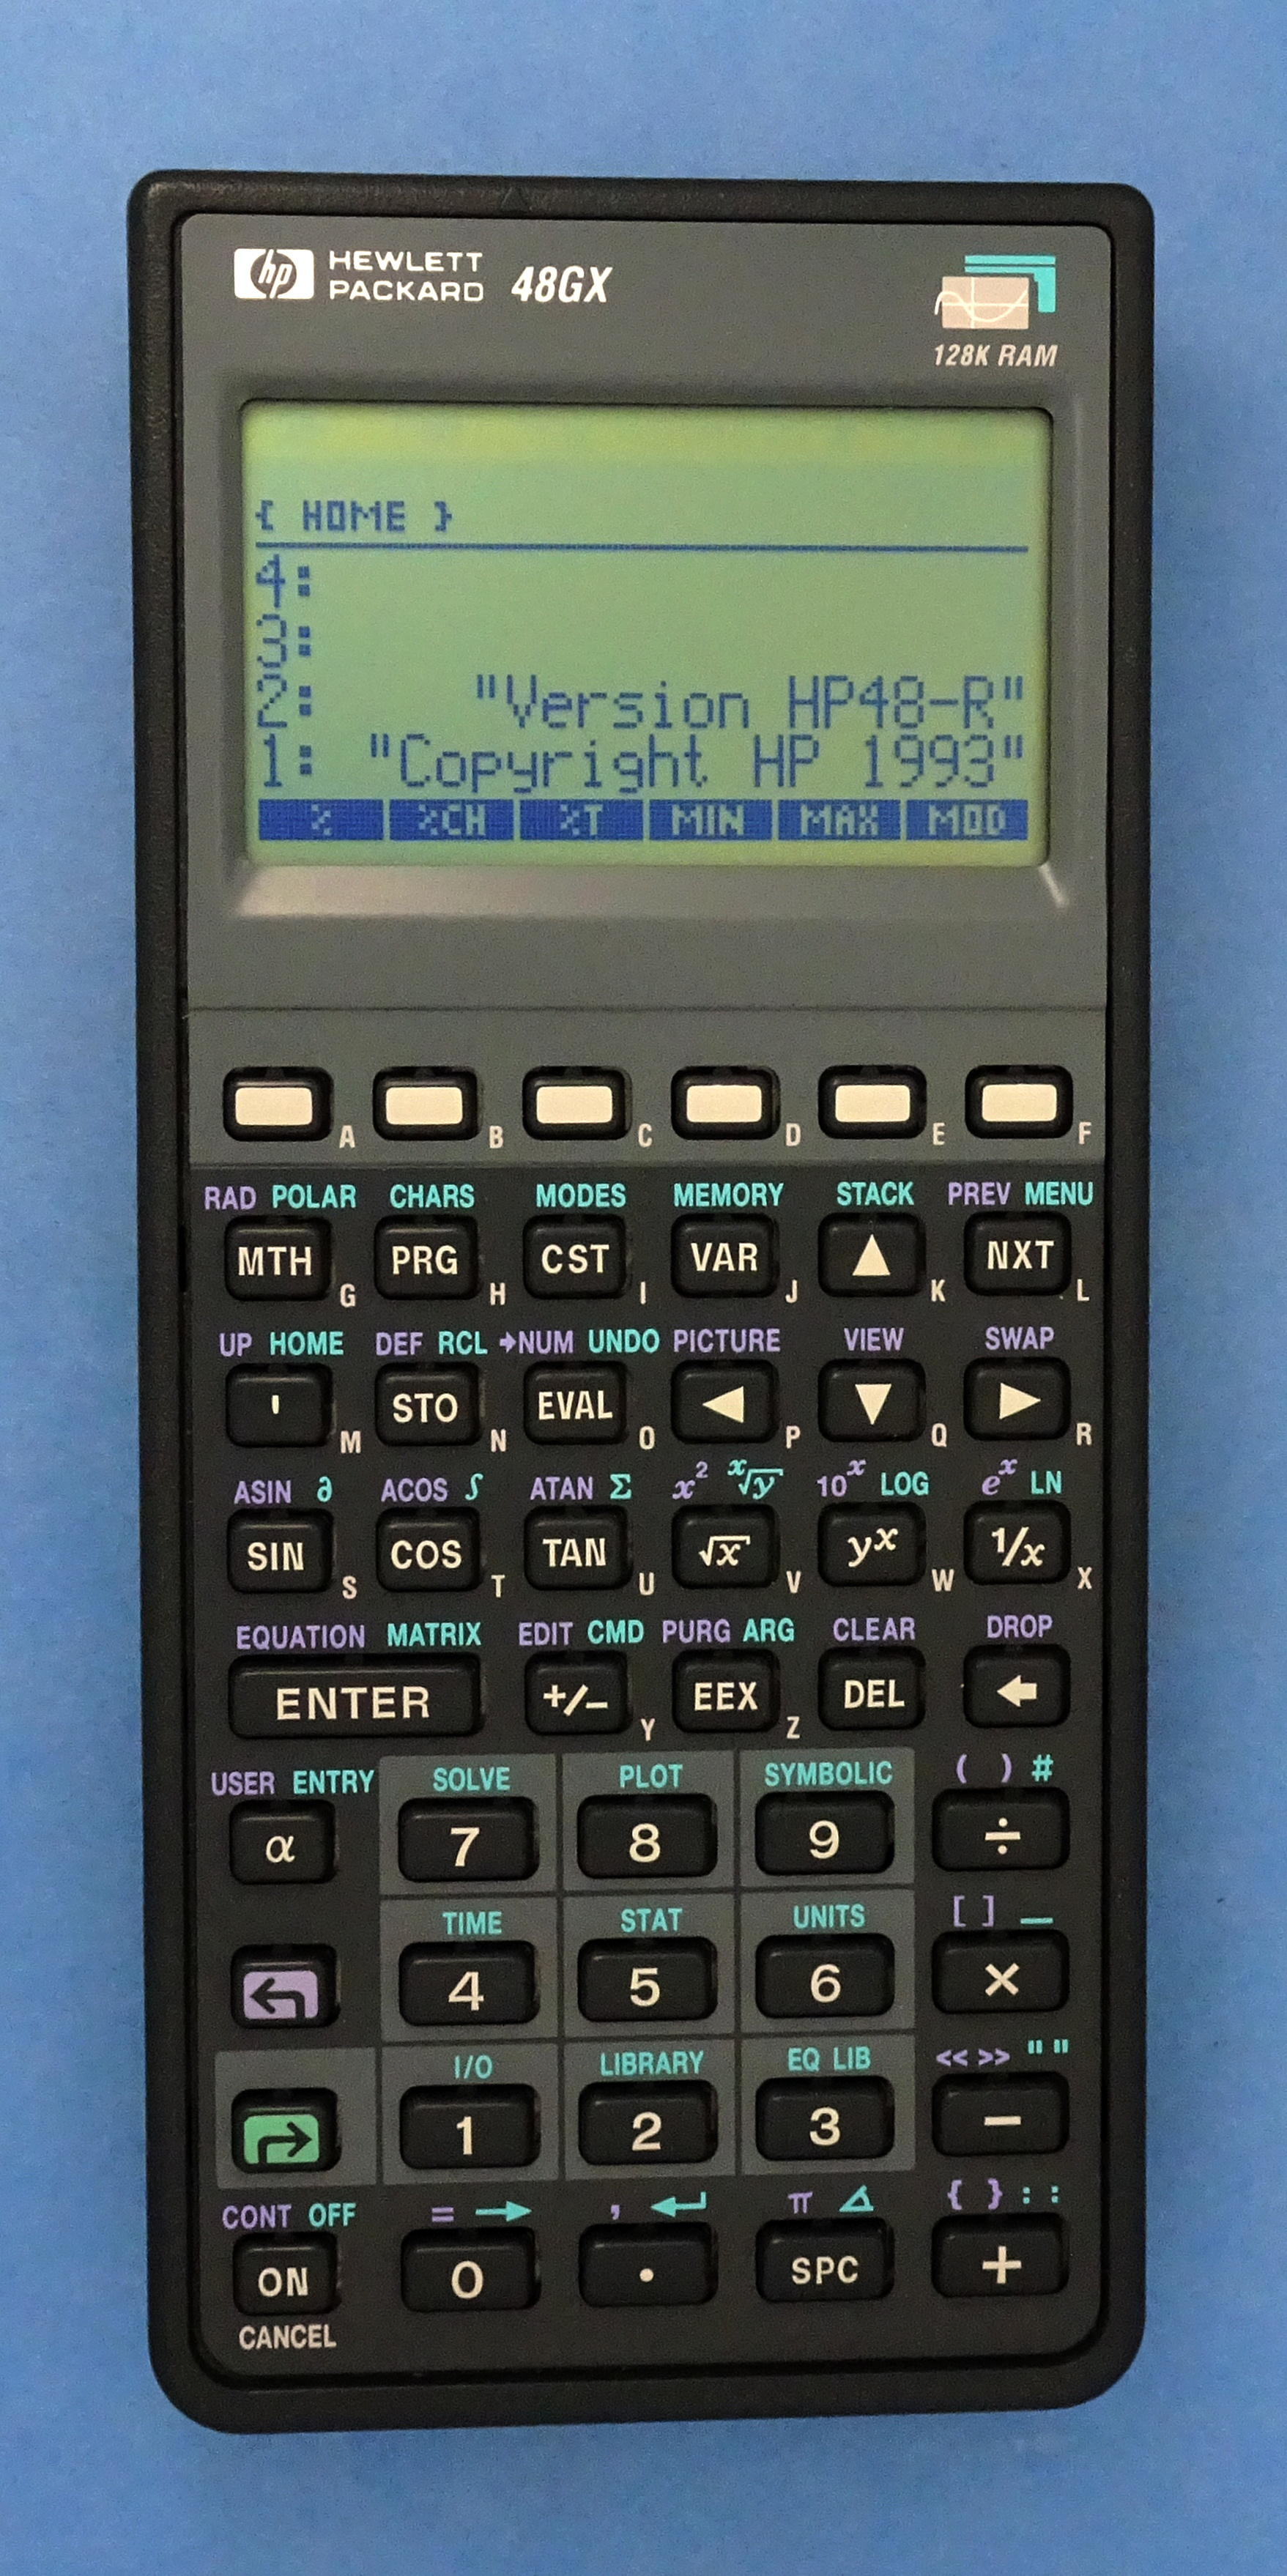
\includegraphics[width=30mm]{hp-calculator.jpg}
            };
        \end{tikzpicture}
    \end{onlyenv}
\end{frame}
\picturecredit{striegel}{HP-48GX calculator}{CC-BY-2.0}{https://flic.kr/p/BWttzE}

\begin{frame}
    \frametitle{Manipulating the stack}
    \stackex<+>{      3 4}{ dup * swap dup * + sqrt }
    \stackex<+>{    3 4 4}{ * swap dup * + sqrt }
    \stackex<+>{     3 16}{ swap dup * + sqrt }
    \stackex<+>{     16 3}{ dup * + sqrt }
    \stackex<+>{   16 3 3}{ * + sqrt }
    \stackex<+>{     16 9}{ + sqrt }
    \stackex<+>{       25}{ sqrt }
    \stackex<+>{        5}{ }
\end{frame}

\begin{frame}
    \frametitle{Abstraction}
    \stackex<+>{         }{ 3 4 \quot{dup * swap dup * + sqrt} apply }
    \stackex<+>{        3}{ 4 \quot{dup * swap dup * + sqrt} apply }
    \stackex<+>{      3 4}{ \quot{dup * swap dup * + sqrt} apply }
    \stackex<+>{      3 4 \quot{dup * swap dup * + sqrt}} { apply }
    \stackex<+>{      3 4}{ dup * swap dup * + sqrt }
    \stackex<+>{    3 4 4}{ * swap dup * + sqrt }
    \stackex<+>{     3 16}{ swap dup * + sqrt }
    \stackex<+>{     16 3}{ dup * + sqrt }
    \stackex<+>{   16 3 3}{ * + sqrt }
    \stackex<+>{     16 9}{ + sqrt }
    \stackex<+>{       25}{ sqrt }
    \stackex<+>{        5}{ }
\end{frame}

\begin{frame}
    \frametitle{Applying a quotation more than once}

    \begin{onlyenv}<+-+(3)>
    \begin{center}
        \stacksplit[only=<+>{colback=gray!20}]{\quot{dup * swap dup * + sqrt}}
        \stacksplit[only=<+>{colback=gray!20}]{dup 3 4 dig2 apply drop}
        \stacksplit[only=<+>{colback=gray!20}]{5 12 dig2 apply drop}
    \end{center}
    \end{onlyenv}

    \stackex<+>{}{ \quot{dup * swap dup * + sqrt} dup 3 4 dig2 apply drop 5 12 dig2 apply drop }
    \stackex<+>{\quot{dup * swap dup * + sqrt}}{ dup 3 4 dig2 apply drop 5 12 dig2 apply drop }
    \stackex<+>{\quot{dup * swap dup * + sqrt} \quot{dup * swap dup * + sqrt}}{ 3 4 dig2 apply drop 5 12 dig2 apply drop }
    \stackex<+>{\quot{dup * swap dup * + sqrt} \quot{dup * swap dup * + sqrt} 3}{ 4 dig2 apply drop 5 12 dig2 apply drop }
    \stackex<+>{\quot{dup * swap dup * + sqrt} \quot{dup * swap dup * + sqrt} 3 4}{ dig2 apply drop 5 12 dig2 apply drop }
    \stackex<+>{\quot{dup * swap dup * + sqrt} 3 4 \quot{dup * swap dup * + sqrt}}{ apply drop 5 12 dig2 apply drop }
    \stackex<+>{\quot{dup * swap dup * + sqrt} 3 4}{ dup * swap dup * + sqrt drop 5 12 dig2 apply drop }
    \stackex<+>{\quot{dup * swap dup * + sqrt} 3 4 4}{ * swap dup * + sqrt drop 5 12 dig2 apply drop }
    \stackex<+>{\quot{dup * swap dup * + sqrt} 3 16}{ swap dup * + sqrt drop 5 12 dig2 apply drop }
    \stackex<+>{\quot{dup * swap dup * + sqrt} 16 3}{ dup * + sqrt drop 5 12 dig2 apply drop }
    \stackex<+>{\quot{dup * swap dup * + sqrt} 16 3 3}{ * + sqrt drop 5 12 dig2 apply drop }
    \stackex<+>{\quot{dup * swap dup * + sqrt} 16 9}{ + sqrt drop 5 12 dig2 apply drop }
    \stackex<+>{\quot{dup * swap dup * + sqrt} 25}{ sqrt drop 5 12 dig2 apply drop }
    \stackex<+>{\quot{dup * swap dup * + sqrt} 5}{ drop 5 12 dig2 apply drop }
    \stackex<+>{\quot{dup * swap dup * + sqrt}}{ 5 12 dig2 apply drop }
    \stackex<+>{\quot{dup * swap dup * + sqrt} 5}{ 12 dig2 apply drop }
    \stackex<+>{\quot{dup * swap dup * + sqrt} 5 12}{ dig2 apply drop }
    \stackex<+>{5 12 \quot{dup * swap dup * + sqrt}}{ apply drop }
    \stackex<+>{5 12}{ dup * swap dup * + sqrt drop }
    \stackex<+>{5 12 12}{ * swap dup * + sqrt drop }
    \stackex<+>{5 144}{ swap dup * + sqrt drop }
    \stackex<+>{144 5}{ dup * + sqrt drop }
    \stackex<+>{144 5 5}{ * + sqrt drop }
    \stackex<+>{144 25}{ + sqrt drop }
    \stackex<+>{169}{ sqrt drop }
    \stackex<+>{13}{ drop }
    \stackex<+>{}{ }
\end{frame}

%%%%%%%%%%%%%%%%%%%%%%%%%%%%%%%%%%%%%%%%%%%%%%%%%%%%%%%%%%%%%%%%%%%%%%%%%%%%%%%%
% Concatenation and composition

\begin{frame}
    \begin{onlyenv}<+-+(1)>
    \begin{center}
        \stacksplit[only=<+>{colback=red!20}]{1 2 + 3 * 2}
        \stacksplit[only=<.>{colback=gray!20}]{2 + 7 3 - *}
        \stacksplit[only=<.>{colback=yellow!20}]{+ sqrt}
    \end{center}
    \end{onlyenv}
\end{frame}

%%%%%%%%%%%%%%%%%%%%%%%%%%%%%%%%%%%%%%%%%%%%%%%%%%%%%%%%%%%%%%%%%%%%%%%%%%%%%%%%

\begin{frame}[t]
    \frametitle{Picture credits}
    \begin{tabular}{lp{0.75\textwidth}}
    \picturecredits
    \end{tabular}
\end{frame}


\end{document}
